\documentclass[11pt,a4paper]{article}
\usepackage[margin=0.8in]{geometry}
\usepackage{amsmath,amssymb}
\usepackage{booktabs}
\usepackage{array}
\usepackage{xcolor}
\usepackage{listings}
\usepackage{graphicx}
\usepackage{tikz}
\usetikzlibrary{arrows.meta,positioning,shapes.geometric,fit,calc}
% hyperref omitted (it needs a LaTeX package that is not installed here)

\lstset{
  basicstyle=\ttfamily\footnotesize,
  breaklines=true,
  frame=single,
  backgroundcolor=\color{gray!5},
  keywordstyle=\color{blue!70!black}\bfseries,
  commentstyle=\color{green!45!black}
}

\title{\textbf{E3: 245 Processor System Design --- Laboratory Exercise 3}\\
\large 5-Stage Pipelined 32-bit RISC-V Processor with Direct-Mapped Instruction Cache}
\author{Anirudh Chaturvedi (SR No: 25850)\\DESE, Indian Institute of Science, Bangalore}
\date{November 2026}

\begin{document}
\maketitle

\section{Introduction \& Design Specifications}
This report documents the design, FPGA implementation, and post-route verification of a \textbf{5-stage pipelined 32-bit RISC-V (RV32I) processor} with a \textbf{direct-mapped Instruction Cache} targeting the Digilent Basys~3 FPGA board (\texttt{XC7A35T-1CPG236C}, Artix-7, speed grade \texttt{-1}).

\begin{itemize}
    \item \textbf{Supported ISA (User Mode):} Basic RV32I arithmetic-logic instructions (R-type and I-type), \texttt{LUI}, branch instructions (\texttt{BEQ}, \texttt{BNE}, \texttt{BLT}, \texttt{BGE}, \texttt{BLTU}, \texttt{BGEU}), load/store instructions (\texttt{LB}, \texttt{LH}, \texttt{LW}, \texttt{LBU}, \texttt{LHU}, \texttt{SB}, \texttt{SH}, \texttt{SW}), and jump instructions (\texttt{JAL}, \texttt{JALR}). Atomic, \texttt{AUIPC}, and CSR instructions are omitted as specified.
    \item \textbf{Pipeline \& Forwarding:} 5-stage pipeline (\textbf{IF, ID, EX, MEM, WB}) with full data forwarding from \textbf{EX/MEM} and \textbf{MEM/WB} outputs to the EX stage (\texttt{forwarding\_unit.v}), plus \textbf{WB-to-ID} write-through bypass in the register file (\texttt{reg\_file.v}).
    \item \textbf{Hazard Detection \& Stall Unit (\texttt{hazard\_unit.v}):} Detects load-use hazards (1-cycle stall of \texttt{PC} and \texttt{IF/ID}, bubble injected into \texttt{ID/EX}), resolves branches/jumps in EX (flushing \texttt{IF/ID} and \texttt{ID/EX}), and freezes all pipeline stages during Instruction Cache misses.
    \item \textbf{Direct-Mapped Instruction Cache (\texttt{icache.v}):} 16 cache lines $\times$ 4 words/block (64 words = 256~bytes), backed by a $512 \times 32$-bit synchronous \textbf{Block RAM} main instruction memory (\texttt{instr\_bram.v}). On a miss, 4 words are fetched sequentially from BRAM without burst transfers.
    \item \textbf{Unaligned Data Memory (\texttt{data\_mem.v}):} 2048-byte memory organized as 4 $\times$ $512 \times 8$-bit Distributed RAM banks supporting single-cycle unaligned byte, half-word, and word transfers.
\end{itemize}

\section{Datapath Block Schematic}
Figure~\ref{fig:datapath} illustrates the 5-stage pipelined RV32I datapath, Instruction Cache hierarchy, forwarding paths, and hazard control signals.

\begin{figure}[htbp]
\centering
\resizebox{\textwidth}{!}{%
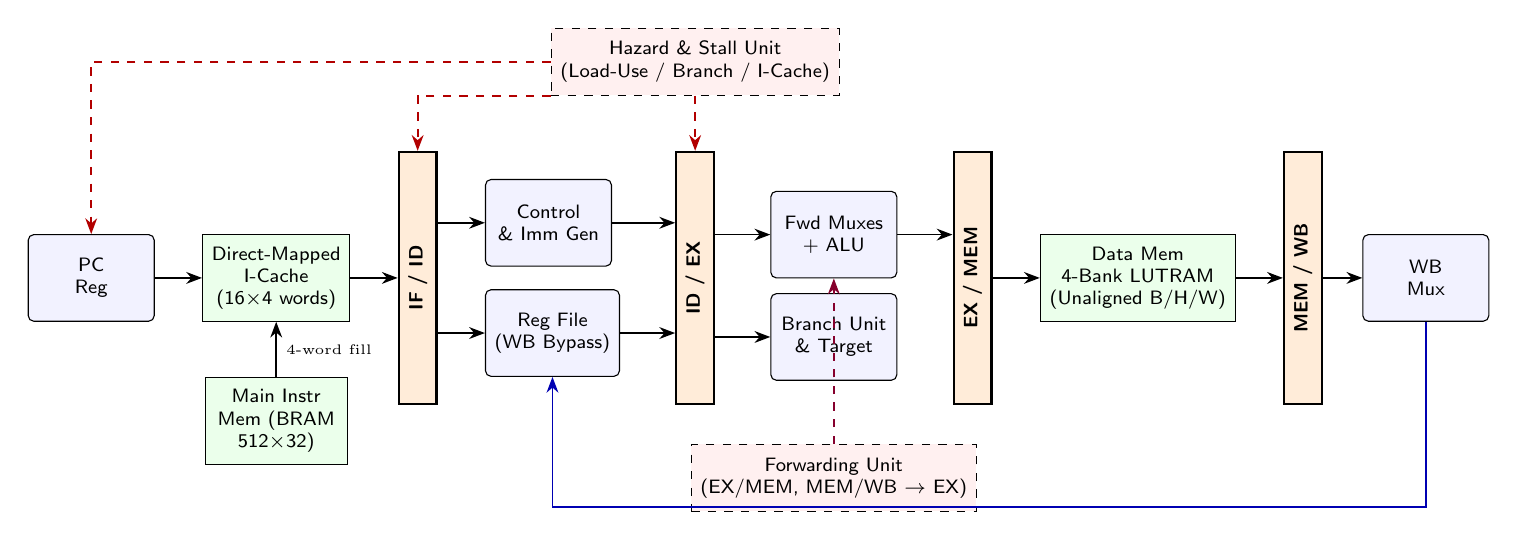
\begin{tikzpicture}[
    node distance=0.85cm and 0.9cm,
    blk/.style={draw, rounded corners=2pt, minimum height=1.1cm, minimum width=1.6cm, align=center, font=\scriptsize\sffamily, fill=blue!5},
    pipe/.style={draw, thick, fill=orange!15, minimum height=3.2cm, minimum width=0.45cm, align=center, font=\scriptsize\bfseries\sffamily},
    mem/.style={draw, fill=green!8, minimum height=1.1cm, minimum width=1.8cm, align=center, font=\scriptsize\sffamily},
    ctrl/.style={draw, dashed, fill=red!6, minimum height=0.85cm, minimum width=2.2cm, align=center, font=\scriptsize\sffamily},
    arr/.style={->, >=Stealth, semithick}
]
% IF Stage
\node[blk] (pc) {PC\\Reg};
\node[mem, right=0.6cm of pc] (ic) {Direct-Mapped\\I-Cache\\(16$\times$4 words)};
\node[mem, below=0.7cm of ic] (bram) {Main Instr\\Mem (BRAM\\512$\times$32)};

% IF/ID
\node[pipe, right=0.6cm of ic] (ifid) {\rotatebox{90}{IF / ID}};

% ID Stage
\node[blk, right=0.6cm of ifid, yshift=0.7cm] (cu) {Control\\\& Imm Gen};
\node[blk, right=0.6cm of ifid, yshift=-0.7cm] (rf) {Reg File\\(WB Bypass)};

% ID/EX
\node[pipe, right=0.7cm of rf, yshift=0.7cm] (idex) {\rotatebox{90}{ID / EX}};

% EX Stage
\node[blk, right=0.7cm of idex, yshift=0.55cm] (alu) {Fwd Muxes\\+ ALU};
\node[blk, right=0.7cm of idex, yshift=-0.75cm] (bru) {Branch Unit\\\& Target};

% EX/MEM
\node[pipe, right=0.7cm of alu, yshift=-0.55cm] (exmem) {\rotatebox{90}{EX / MEM}};

% MEM Stage
\node[mem, right=0.6cm of exmem] (dmem) {Data Mem\\4-Bank LUTRAM\\(Unaligned B/H/W)};

% MEM/WB
\node[pipe, right=0.6cm of dmem] (memwb) {\rotatebox{90}{MEM / WB}};

% WB Stage
\node[blk, right=0.5cm of memwb] (wb) {WB\\Mux};

% Hazard & Forwarding
\node[ctrl, above=0.7cm of idex] (haz) {Hazard \& Stall Unit\\(Load-Use / Branch / I-Cache)};
\node[ctrl, below=0.8cm of bru] (fwd) {Forwarding Unit\\(EX/MEM, MEM/WB $\rightarrow$ EX)};

% Connections
\draw[arr] (pc) -- (ic);
\draw[arr] (bram) -- node[right,font=\tiny]{4-word fill} (ic);
\draw[arr] (ic) -- (ifid);
\draw[arr] (ifid.east |- cu.west) -- (cu.west);
\draw[arr] (ifid.east |- rf.west) -- (rf.west);
\draw[arr] (cu.east) -- (idex.west |- cu.east);
\draw[arr] (rf.east) -- (idex.west |- rf.east);
\draw[arr] (idex.east |- alu.west) -- (alu.west);
\draw[arr] (idex.east |- bru.west) -- (bru.west);
\draw[arr] (alu.east) -- (exmem.west |- alu.east);
\draw[arr] (exmem) -- (dmem);
\draw[arr] (dmem) -- (memwb);
\draw[arr] (memwb) -- (wb);

% Feedback paths
\draw[arr, blue!70!black] (wb.south) -- ++(0,-2.35) -| (rf.south);
\draw[arr, red!70!black, dashed] (haz.west) -| (pc.north);
\draw[arr, red!70!black, dashed] (haz.south west) -| (ifid.north);
\draw[arr, red!70!black, dashed] (haz.south) -- (idex.north);
\draw[arr, purple!70!black, dashed] (fwd.north) -- (alu.south);
\end{tikzpicture}
}
\caption{5-Stage Pipelined RV32I Processor with Direct-Mapped Instruction Cache.}
\label{fig:datapath}
\end{figure}

\begin{table}[htbp]
\centering
\caption{Direct-Mapped Instruction Cache Address Decomposition (32-bit Byte Address)}
\begin{tabular}{@{}cccc@{}}
\toprule
\textbf{Bits [31:8] (24 bits)} & \textbf{Bits [7:4] (4 bits)} & \textbf{Bits [3:2] (2 bits)} & \textbf{Bits [1:0] (2 bits)} \\ \midrule
Tag & Cache Index (0--15) & Word Offset (0--3) & Byte Offset (\texttt{00}) \\ \bottomrule
\end{tabular}
\end{table}

\subsection*{RTL schematic (Vivado elaborated design)}
Figure~\ref{fig:rtlschem} is the schematic Vivado 2026.1 generates after elaboration (\textit{RTL Analysis $\rightarrow$ Open Elaborated Design $\rightarrow$ Schematic}). The top level \texttt{basys3\_top} contains the processor \texttt{u\_cpu} (\texttt{rv32i\_pipeline\_cpu}), the seven-segment driver \texttt{u\_seg7}, and a 4:1 output multiplexer (\texttt{disp\_val\_i}) that selects which 16-bit value drives the LEDs from \texttt{sw[1:0]} (quotient, remainder, \texttt{pc\_out}, status flags). Figure~\ref{fig:rtlschem_cpu} shows the same design with \texttt{u\_cpu} expanded (711 cells, 1,704 nets).

\begin{figure}[htbp]
\centering
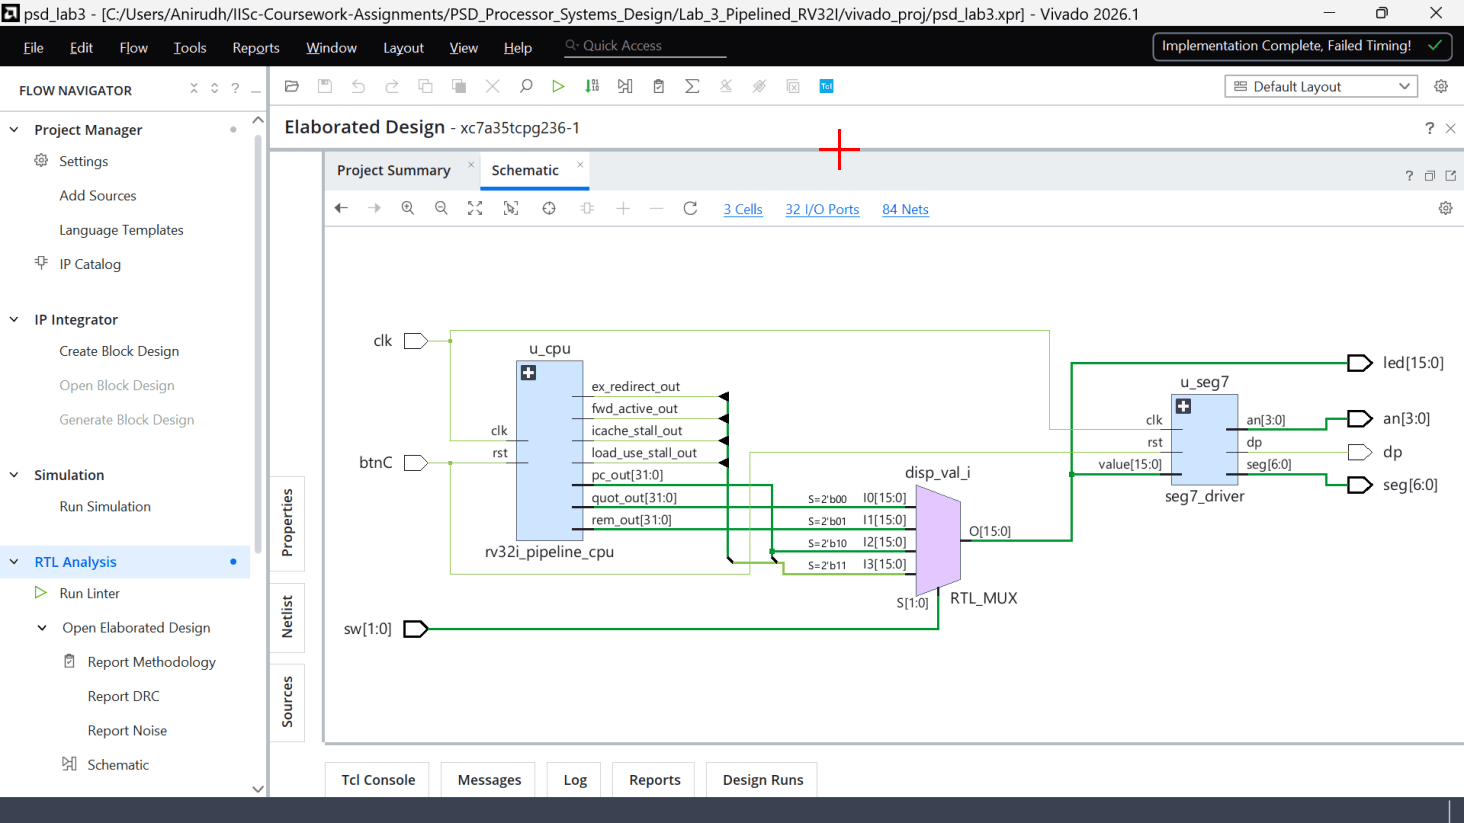
\includegraphics[width=\textwidth]{figures/fig_rtl_schematic_top.png}
\caption{Vivado RTL schematic, top level: \texttt{u\_cpu}, \texttt{u\_seg7} and the \texttt{sw[1:0]}-controlled output multiplexer.}
\label{fig:rtlschem}
\end{figure}

\begin{figure}[htbp]
\centering
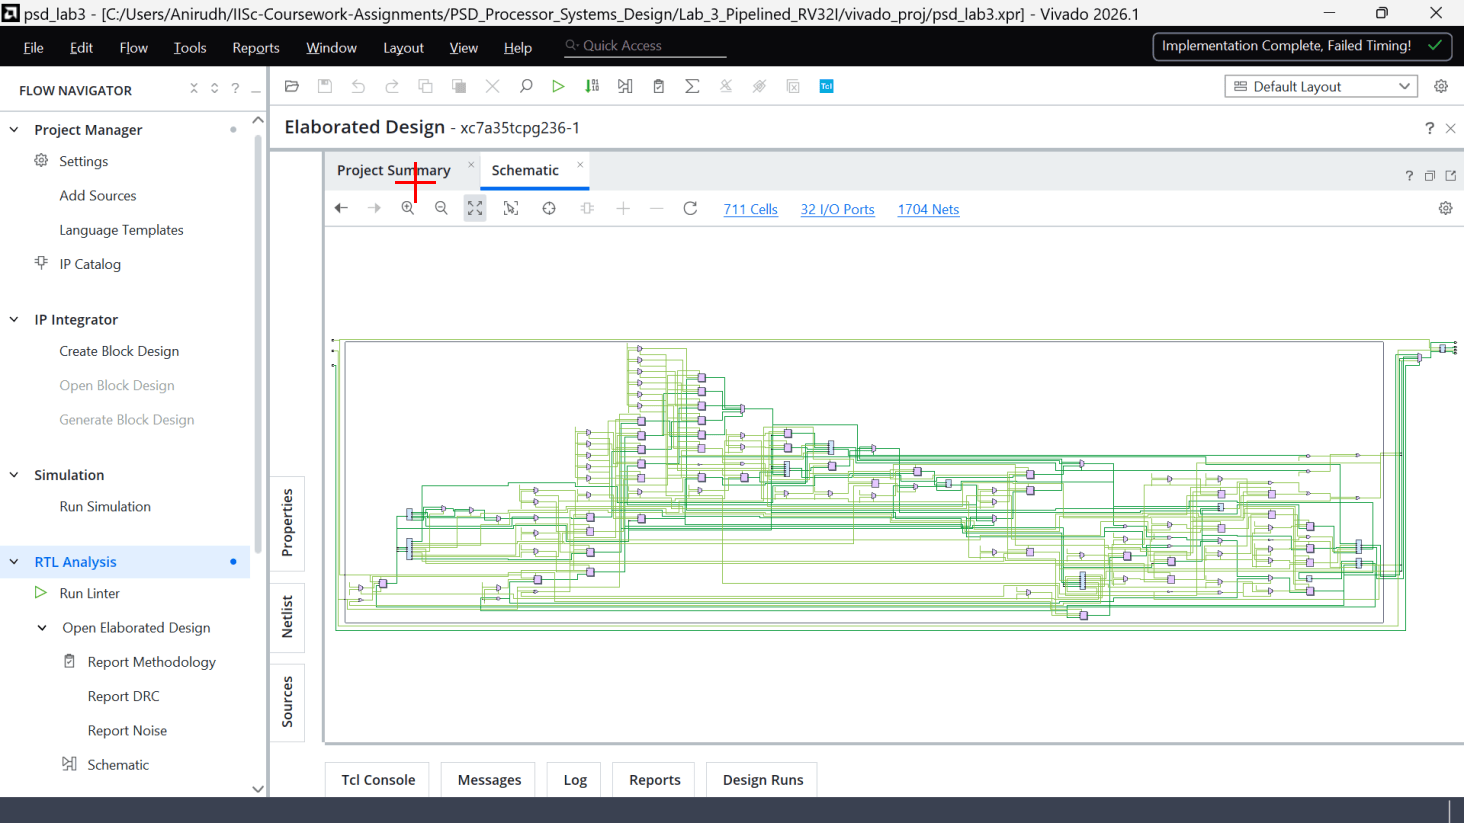
\includegraphics[width=\textwidth]{figures/fig_rtl_schematic_cpu_expanded.png}
\caption{Vivado RTL schematic with \texttt{u\_cpu} expanded (711 cells, 1,704 nets).}
\label{fig:rtlschem_cpu}
\end{figure}

\section{Controller \& I-Cache FSM State Diagram}
Figure~\ref{fig:fsm} shows the Instruction Cache miss/fill controller FSM, and Table~\ref{tab:hazard} summarizes the pipeline stall and flush truth table.

\begin{figure}[htbp]
\centering
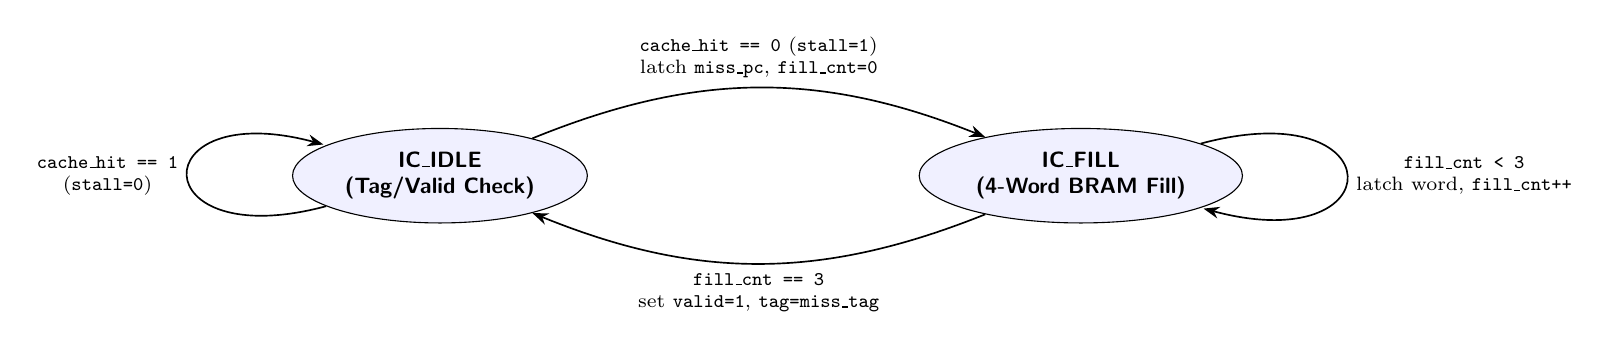
\begin{tikzpicture}[
    node distance=4.2cm,
    st/.style={draw, ellipse, minimum width=2.5cm, minimum height=1.2cm, align=center, font=\footnotesize\bfseries\sffamily, fill=blue!6},
    arr/.style={->, >=Stealth, semithick}
]
\node[st] (idle) {IC\_IDLE\\(Tag/Valid Check)};
\node[st, right=of idle] (fill) {IC\_FILL\\(4-Word BRAM Fill)};

\draw[arr] (idle) edge[loop left] node[left, align=center, font=\scriptsize]{\texttt{cache\_hit == 1}\\(\texttt{stall=0})} (idle);
\draw[arr] (idle) edge[bend left=22] node[above, align=center, font=\scriptsize]{\texttt{cache\_hit == 0} (\texttt{stall=1})\\latch \texttt{miss\_pc}, \texttt{fill\_cnt=0}} (fill);
\draw[arr] (fill) edge[loop right] node[right, align=center, font=\scriptsize]{\texttt{fill\_cnt < 3}\\latch word, \texttt{fill\_cnt++}} (fill);
\draw[arr] (fill) edge[bend left=22] node[below, align=center, font=\scriptsize]{\texttt{fill\_cnt == 3}\\set \texttt{valid=1}, \texttt{tag=miss\_tag}} (idle);
\end{tikzpicture}
\caption{Instruction Cache Miss/Fill Controller FSM.}
\label{fig:fsm}
\end{figure}

\begin{table}[htbp]
\centering
\caption{Hazard Detection \& Pipeline Stall/Flush Control Truth Table}
\begin{tabular}{@{}lcccc@{}}
\toprule
\textbf{Condition} & \texttt{stall\_if/id} & \texttt{stall\_ex/mem/wb} & \texttt{flush\_if\_id} & \texttt{flush\_id\_ex} \\ \midrule
\texttt{icache\_stall == 1} & 1 & 1 & 0 & 0 \\
\texttt{ex\_redirect == 1} (Branch/JAL/JALR) & 0 & 0 & 1 & 1 \\
\texttt{load\_use\_stall == 1} & 1 & 0 & 0 & 1 \\
Normal Execution & 0 & 0 & 0 & 0 \\ \bottomrule
\end{tabular}
\label{tab:hazard}
\end{table}

\section{Verification: 16-bit Unsigned Restoring Division}
The processor was tested with a C/RISC-V assembly program (\texttt{restoring\_div.c}, \texttt{restoring\_div.asm}) implementing \texttt{restoring\_divide(100, 7, \&rem)} as a function called via \texttt{jal ra, restoring\_divide} and returning via \texttt{jalr x0, ra, 0}, followed by unaligned byte/half-word/word memory tests and a back-to-back load-use hazard.

\begin{table}[htbp]
\centering
\caption{Behavioral (\texttt{iverilog}) and Post-Route Timing (\texttt{xsim}) Verification Results}
\begin{tabular}{@{}lll@{}}
\toprule
\textbf{Check / Metric} & \textbf{Observed Value} & \textbf{Status} \\ \midrule
Quotient \texttt{MEM[0x200]} ($100 / 7$) & \texttt{14} (\texttt{0x0000000E}) & PASS (Behavioral \& Post-Route) \\
Remainder \texttt{MEM[0x204]} ($100 \bmod 7$) & \texttt{2} (\texttt{0x00000002}) & PASS (Behavioral \& Post-Route) \\
Unaligned \texttt{MEM[0x208]} (\texttt{sb}/\texttt{sh}) & \texttt{0xC0DE5A00} & PASS \\
Unaligned + Load-Use \texttt{MEM[0x210]} & \texttt{0x00C0DE5B} & PASS \\
I-Cache Misses / Stall Cycles & 10 misses / 50 stall cycles & Verified (5 cycles/miss) \\
Load-Use Stalls / Branch Flushes / Fwd & 1 stall / 106 flushes / 73 fwd & Verified \\ \bottomrule
\end{tabular}
\end{table}

\subsection*{Behavioral simulation waveforms (Vivado Simulator)}
The testbench \texttt{rv32i\_pipeline\_tb} runs 500 clock cycles at 100~MHz, counts I-cache misses, stall cycles, flushes and forwarding events, checks the stored results, and prints the summary of Figure~\ref{fig:consolebehav}.

\begin{figure}[htbp]
\centering
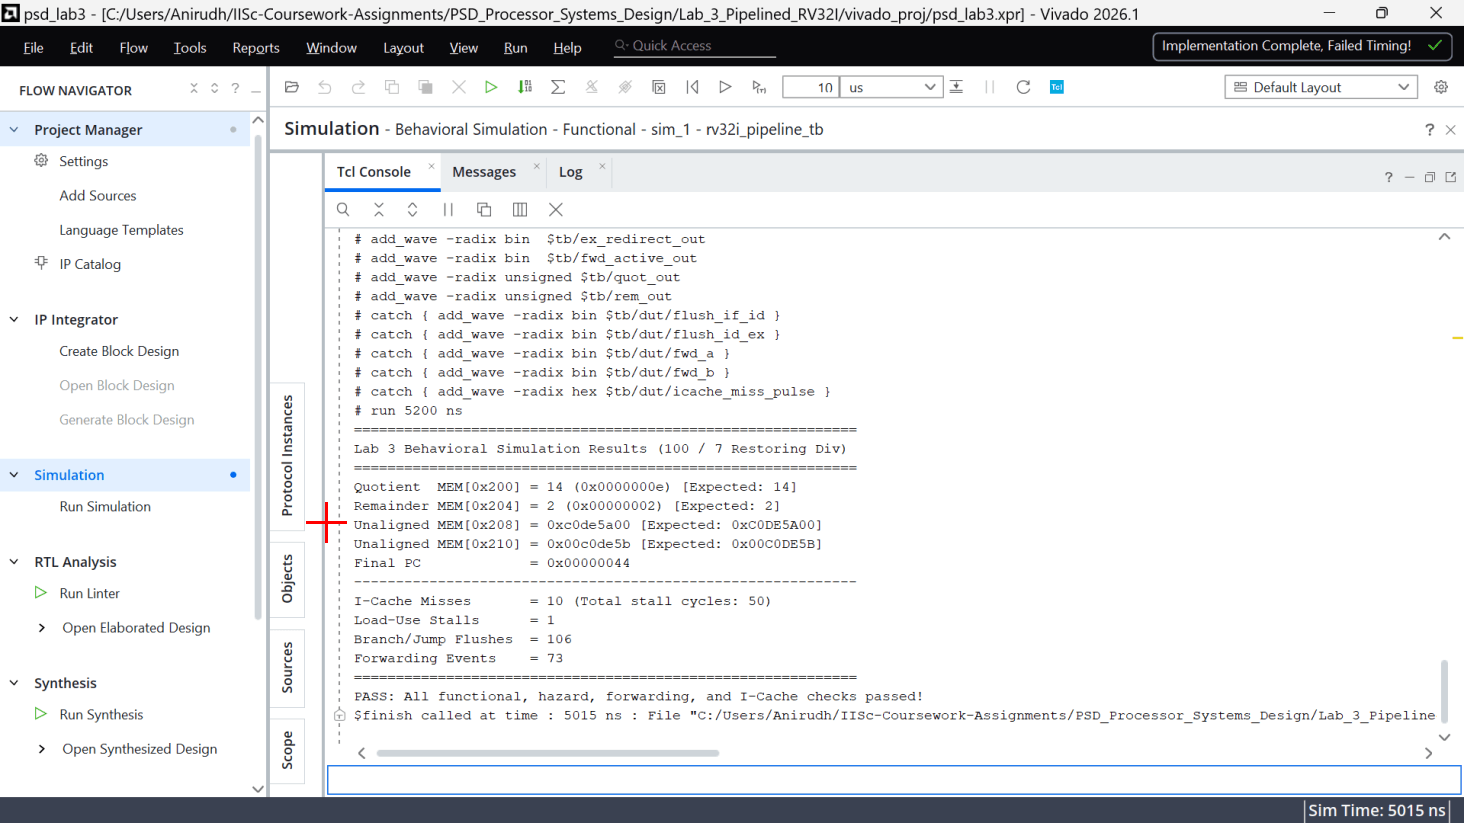
\includegraphics[width=\textwidth]{figures/fig_console_behav_summary.png}
\caption{Vivado Tcl console after behavioral simulation: quotient 14, remainder 2, both unaligned-access checks pass, 10 I-cache misses (50 stall cycles), 1 load-use stall, 106 branch/jump flushes, 73 forwarding events; simulation ends at 5,015~ns.}
\label{fig:consolebehav}
\end{figure}

\begin{figure}[htbp]
\centering
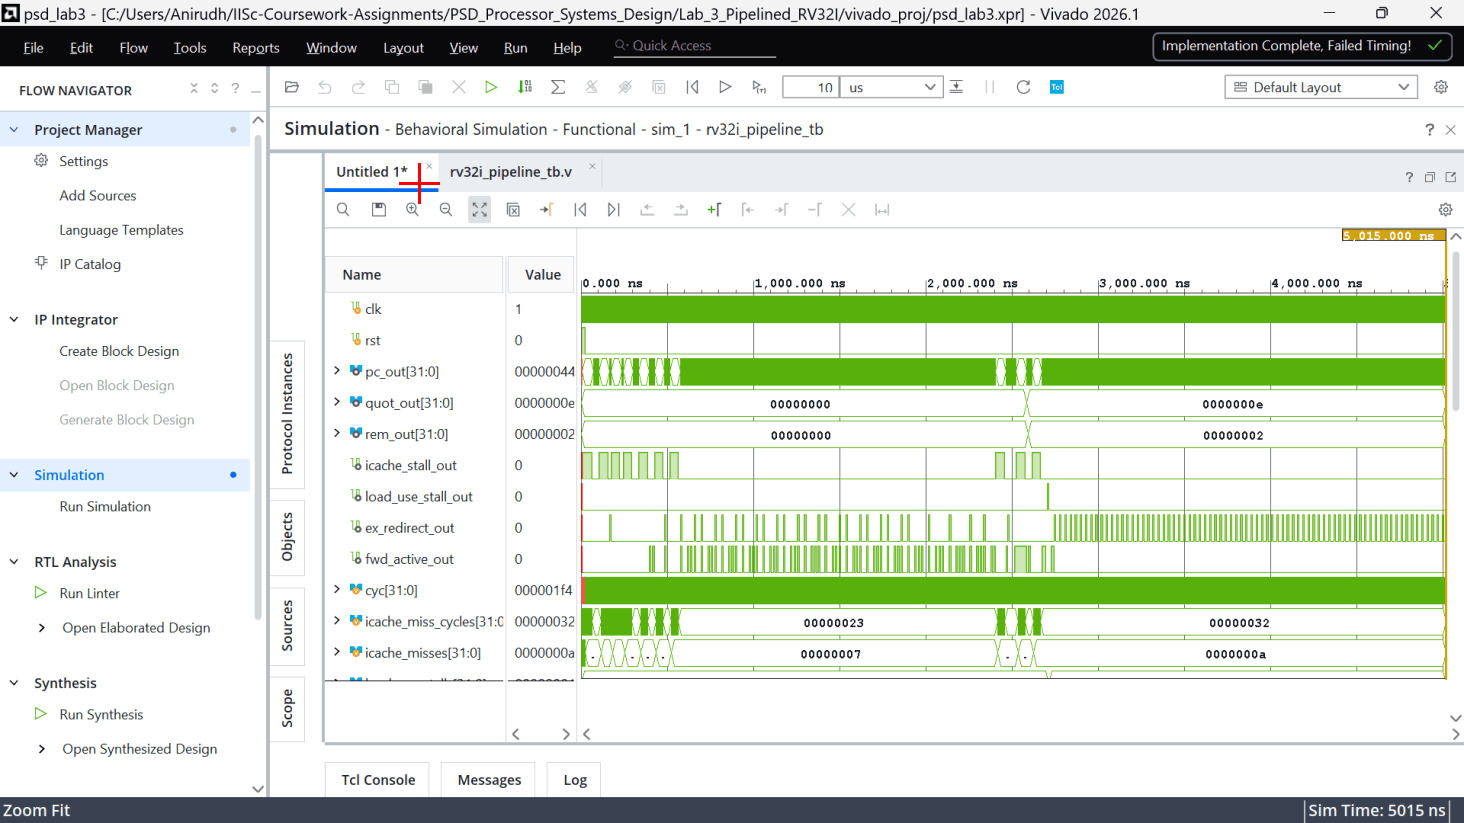
\includegraphics[width=\textwidth]{figures/fig_wave_behav_full.png}
\caption{Behavioral simulation, full run (0--5,015~ns). \texttt{icache\_stall\_out} pulses are the I-cache misses (cold start and a second burst near 2.6~\textmu s); \texttt{ex\_redirect\_out} and \texttt{fwd\_active\_out} show branch/jump flushes and forwarding; \texttt{quot\_out} and \texttt{rem\_out} become \texttt{0x0e} and \texttt{0x02} by about 2.6~\textmu s.}
\label{fig:wavefull}
\end{figure}

\begin{figure}[htbp]
\centering
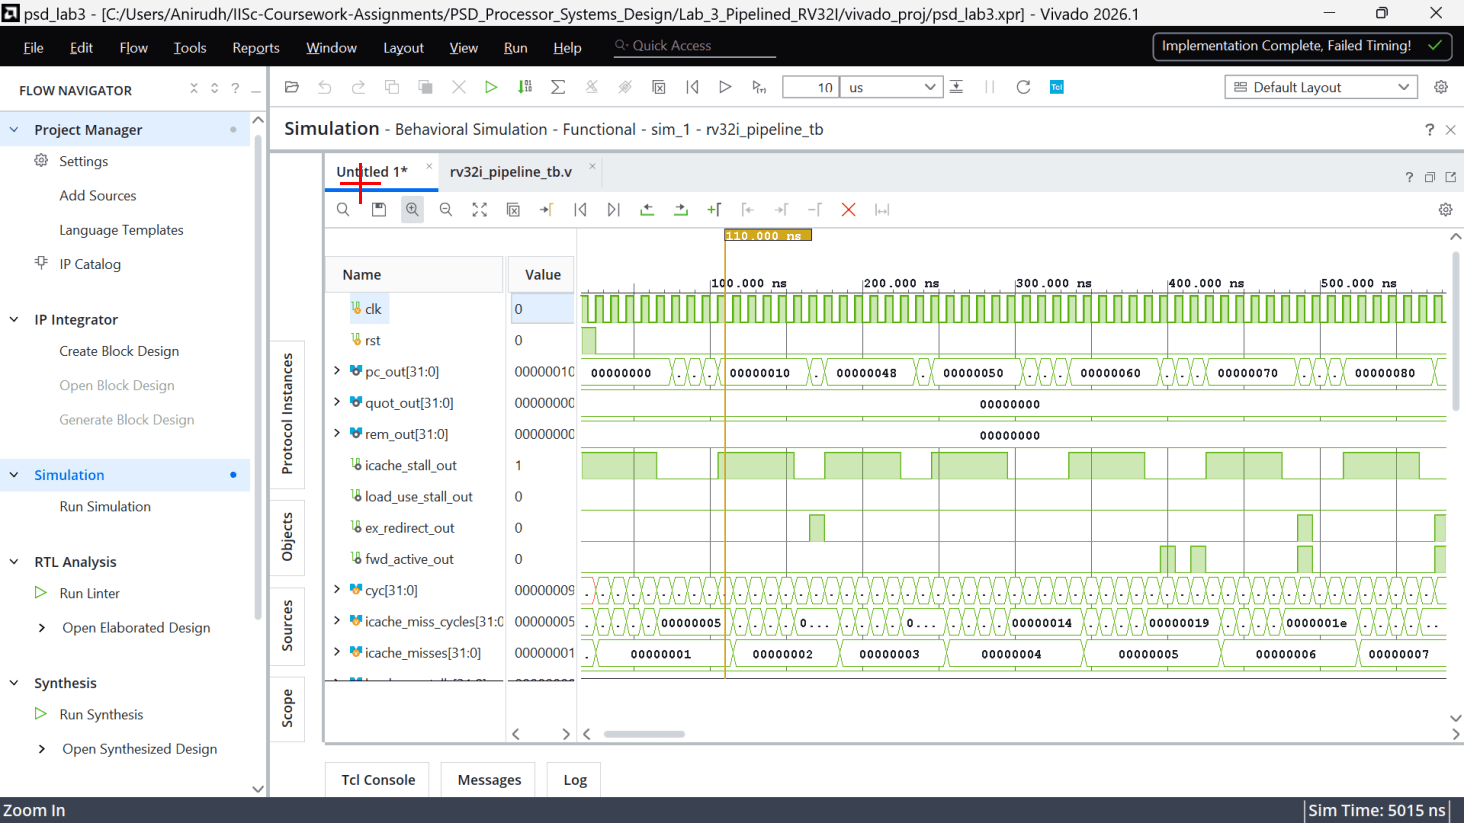
\includegraphics[width=\textwidth]{figures/fig_wave_icache_miss.png}
\caption{Instruction-cache misses and block fills (0--550~ns). Each miss asserts \texttt{icache\_stall\_out} for five cycles (50~ns) while \texttt{pc\_out} is frozen; \texttt{icache\_misses} counts 1 to 7 and \texttt{icache\_miss\_cycles} steps in units of five (\texttt{0x05}, \texttt{0x14}, \texttt{0x19}, \texttt{0x1e}). \texttt{ex\_redirect\_out} pulses (branch/jump flush) appear near 170~ns and 490~ns, and \texttt{fwd\_active\_out} pulses near 400--430~ns.}
\label{fig:wavemiss}
\end{figure}

\begin{figure}[htbp]
\centering
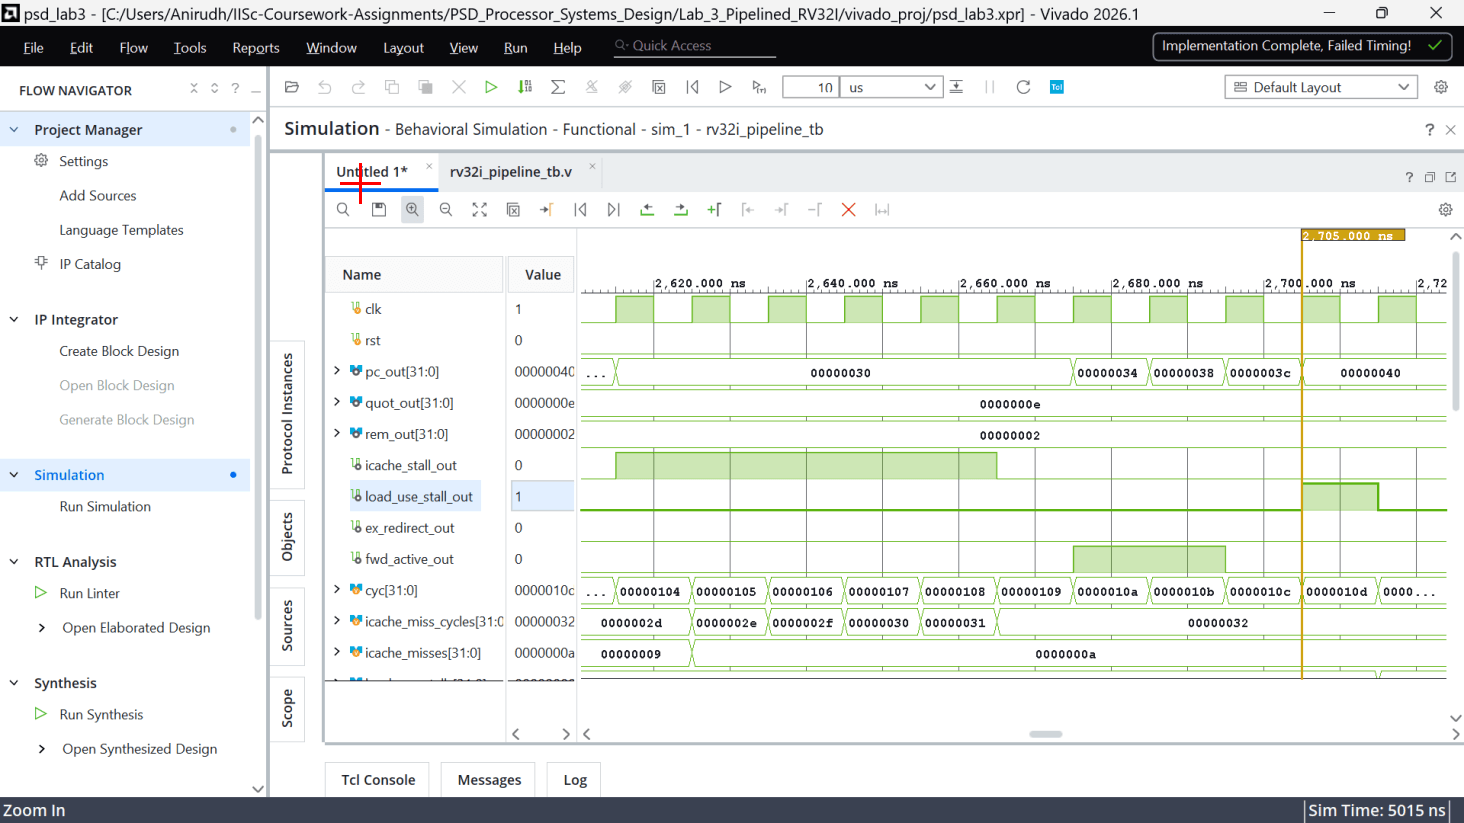
\includegraphics[width=\textwidth]{figures/fig_wave_loaduse_miss_fwd.png}
\caption{Cache miss, forwarding and the load-use stall (about 2,610--2,730~ns). A five-cycle I-cache stall (about 2,615--2,665~ns) holds \texttt{pc\_out} at \texttt{0x30}; \texttt{fwd\_active\_out} marks a forwarding event (about 2,675--2,695~ns); \texttt{load\_use\_stall\_out} is high for one cycle at 2,705--2,715~ns (cursor), the single load-use stall in this program.}
\label{fig:waveloaduse}
\end{figure}

\begin{figure}[htbp]
\centering
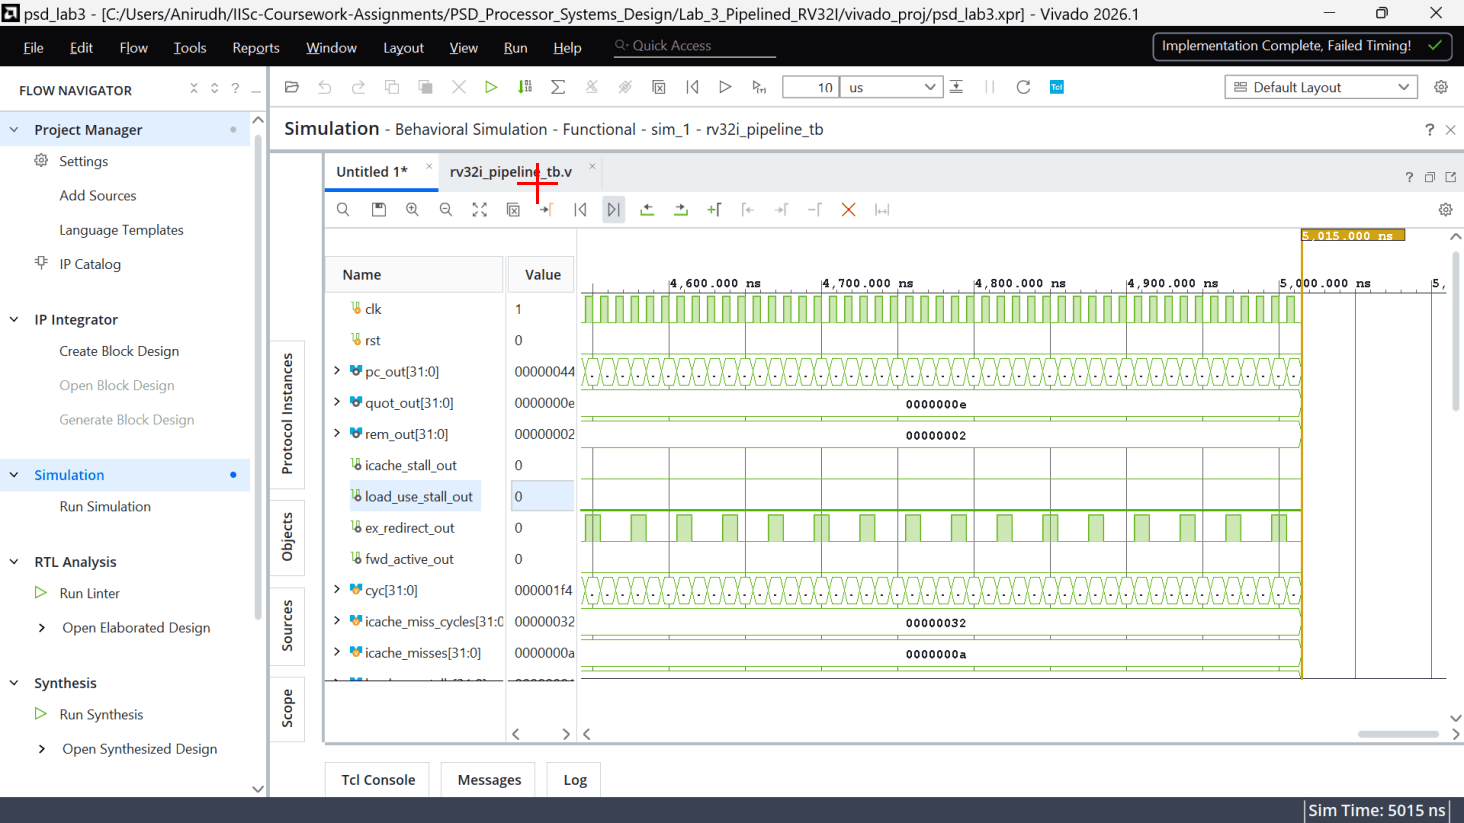
\includegraphics[width=\textwidth]{figures/fig_wave_result_behav.png}
\caption{End of the behavioral run (about 4.6--5.0~\textmu s): \texttt{quot\_out} $=$ \texttt{0x0e} (14) and \texttt{rem\_out} $=$ \texttt{0x02} (2) are stable while the program idles in its final loop (\texttt{ex\_redirect\_out} pulses on every jump).}
\label{fig:waveresult}
\end{figure}

\subsection*{Post-route timing simulation (with SDF back-annotation)}
The same program was run on the post-implementation netlist with the SDF file written by Vivado (\textit{Run Simulation $\rightarrow$ Run Post-Implementation Timing Simulation}), using the top-level testbench \texttt{basys3\_top\_tb}: reset is released after 100~ns (GSR), the program runs for 5,000~ns, then \texttt{sw}$=$\texttt{00} selects the quotient and \texttt{sw}$=$\texttt{01} the remainder on the LEDs.

\begin{figure}[htbp]
\centering
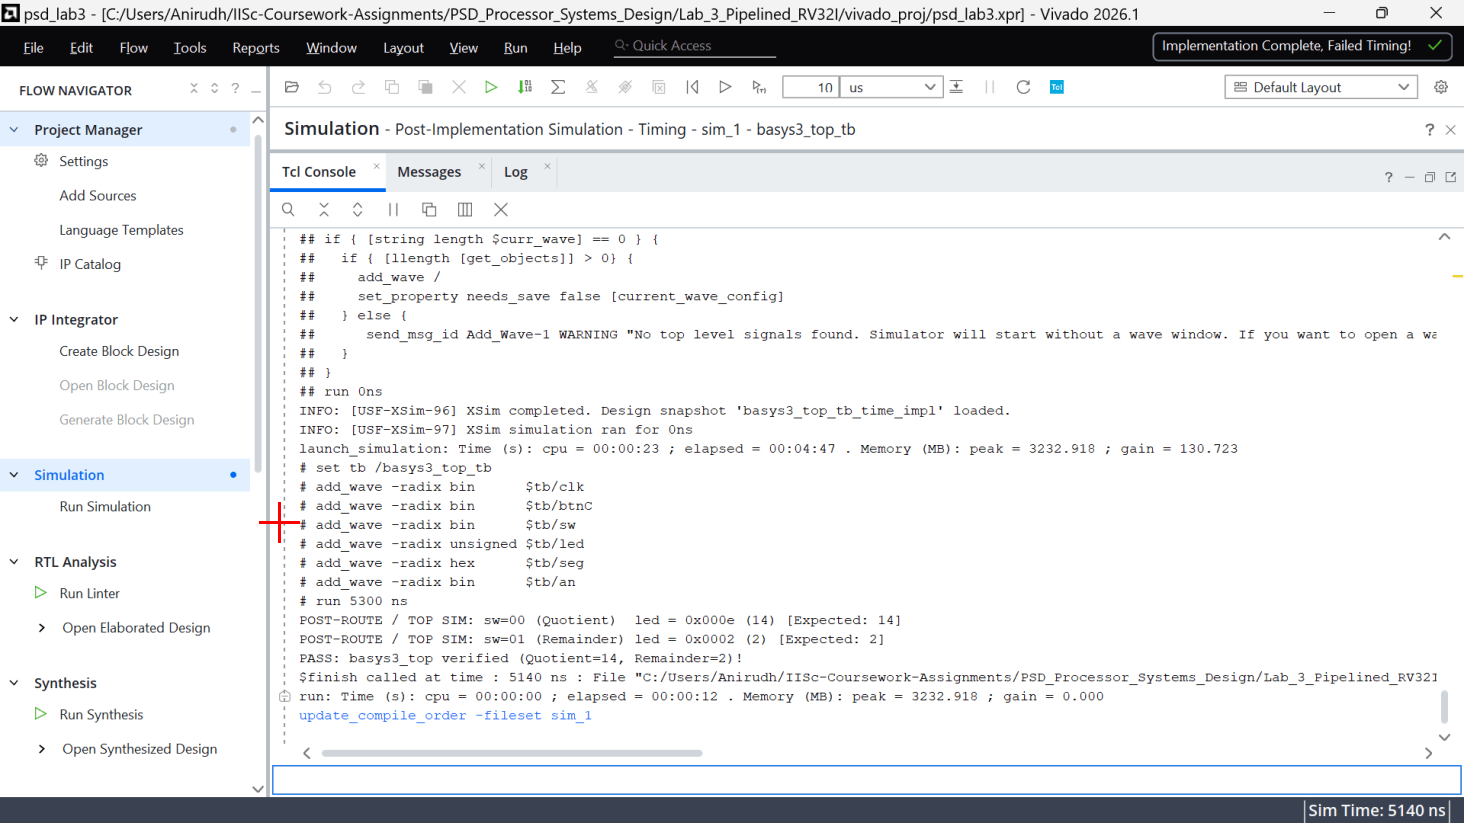
\includegraphics[width=\textwidth]{figures/fig_console_postroute.png}
\caption{Post-route timing simulation log: \texttt{sw}$=$\texttt{00} gives \texttt{led} $=$ \texttt{0x000e} (14), \texttt{sw}$=$\texttt{01} gives \texttt{led} $=$ \texttt{0x0002} (2); ``PASS: basys3\_top verified''; simulation ends at 5,140~ns.}
\label{fig:consolepost}
\end{figure}

\begin{figure}[htbp]
\centering
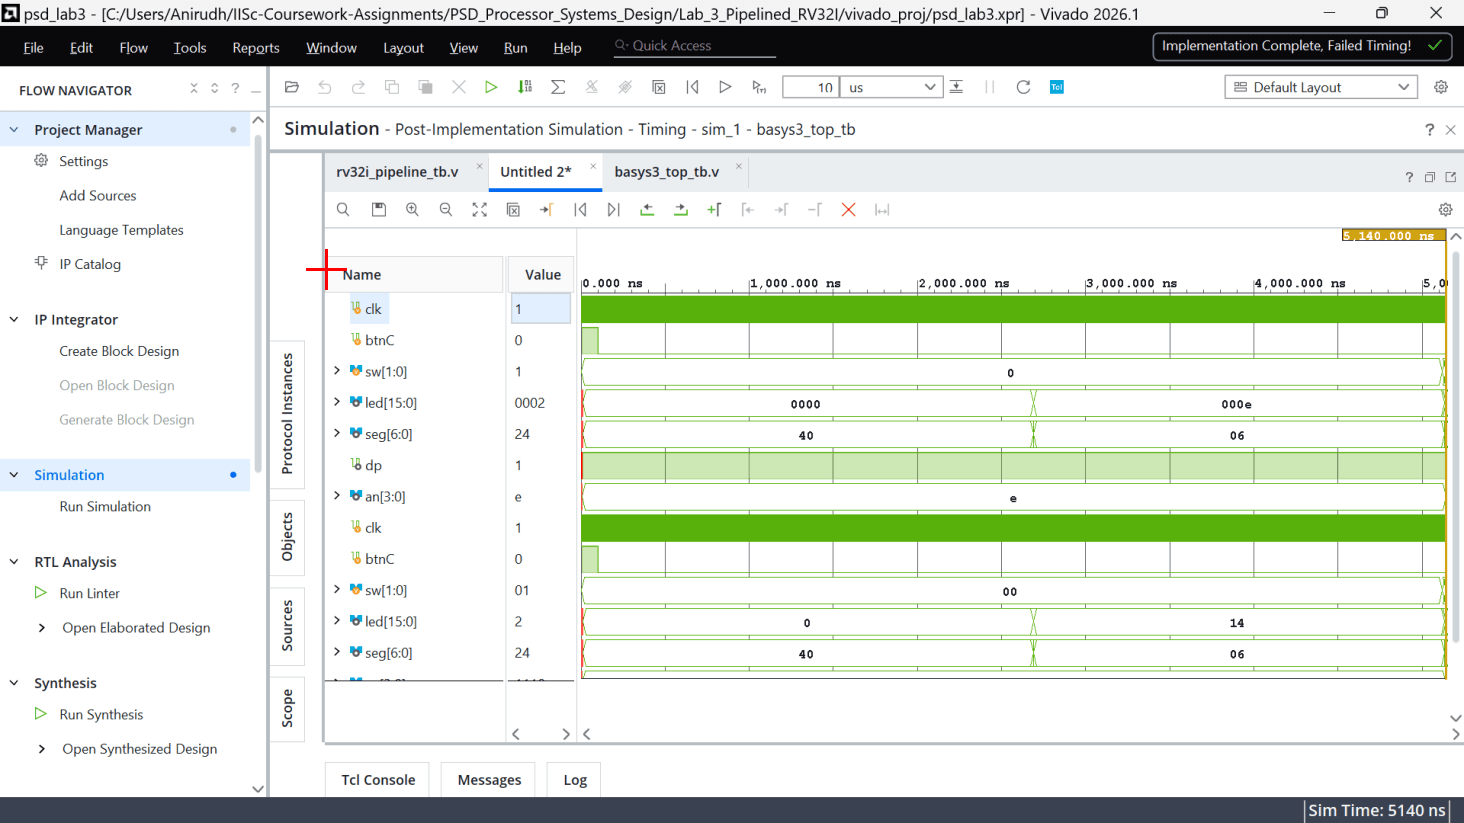
\includegraphics[width=\textwidth]{figures/fig_wave_postroute_full.png}
\caption{Post-route timing simulation, full run (0--5,140~ns). \texttt{led} (shown in hex above, in decimal below) changes from 0 to \texttt{0x000e} once the program has stored the quotient (about 2.7~\textmu s) while \texttt{sw}$=$\texttt{00}.}
\label{fig:postfull}
\end{figure}

\begin{figure}[htbp]
\centering
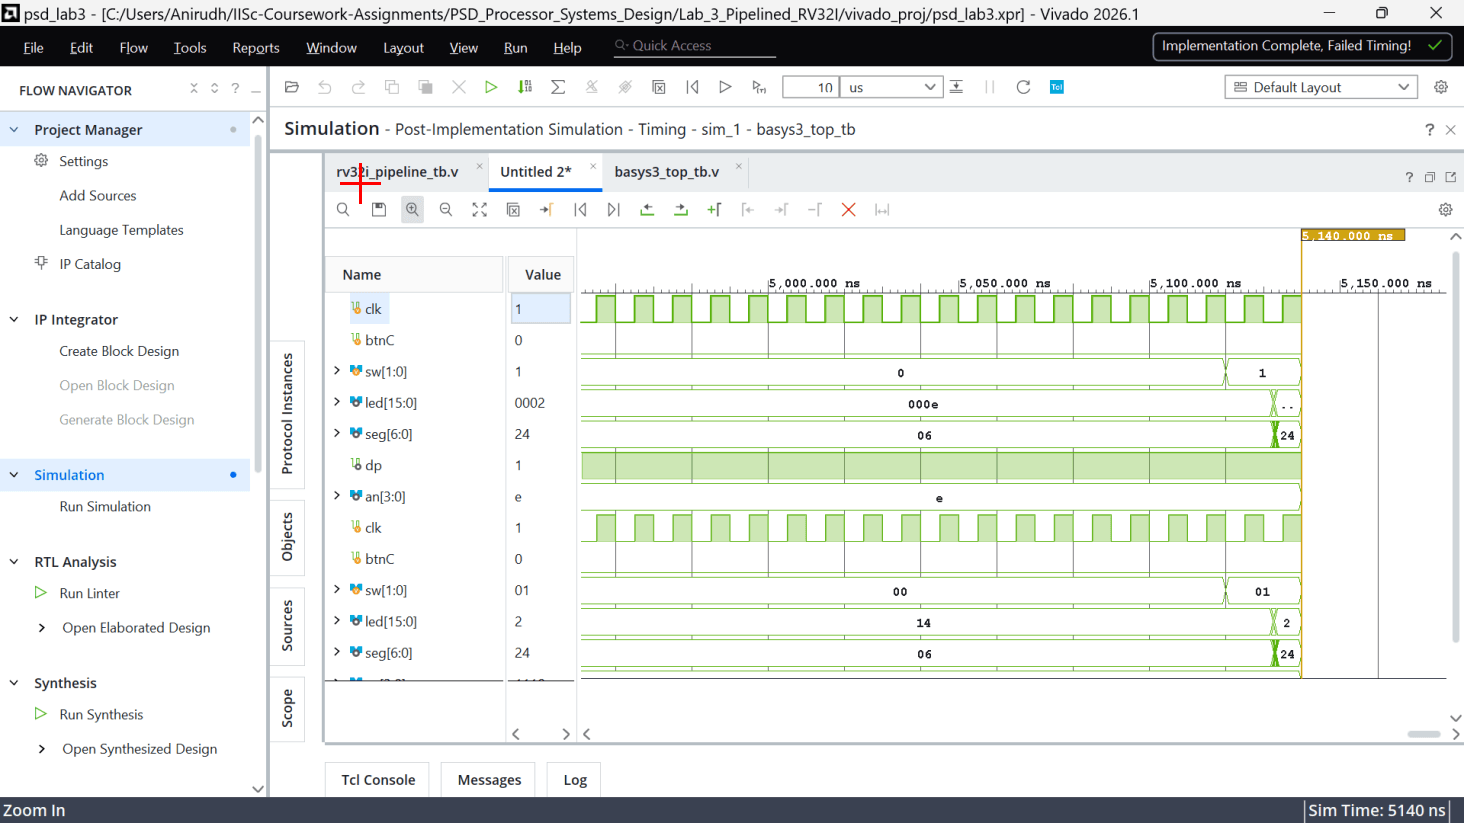
\includegraphics[width=\textwidth]{figures/fig_wave_postroute_result.png}
\caption{Post-route timing simulation, 5,000--5,140~ns. At about 5,120~ns \texttt{sw} changes from \texttt{00} to \texttt{01}; \texttt{led} changes from \texttt{0x000e} (14) to \texttt{0x0002} (2) after a short unknown interval caused by the back-annotated gate and routing delays, and \texttt{seg} changes from \texttt{06} to \texttt{24}.}
\label{fig:postresult}
\end{figure}

\section{Vivado 2026.1 Post-Route Timing \& Resource Utilization}
The complete design (\texttt{basys3\_top.v}) was synthesized, placed, routed, and verified with post-implementation timing simulation in \textbf{Vivado 2026.1} for \texttt{xc7a35tcpg236-1} with a 100~MHz (\texttt{10.000~ns}) clock constraint.

\begin{table}[htbp]
\centering
\caption{Post-Route Resource Utilization and Timing Summary (\texttt{xc7a35tcpg236-1})}
\resizebox{\textwidth}{!}{%
\begin{tabular}{@{}lrrr@{}}
\toprule
\textbf{Resource / Timing Metric} & \textbf{Used / Value} & \textbf{Available / Target} & \textbf{Utilization / Margin} \\ \midrule
Slice LUTs (Total) & 2,955 & 20,800 & 14.21\% \\
\quad LUT as Logic & 2,699 & 20,800 & 12.98\% \\
\quad LUT as Distributed RAM (\texttt{data\_mem}) & 256 & 9,600 & 2.67\% \\
Slice Registers (Flip-Flops) & 4,165 & 41,600 & 10.01\% \\
Block RAM (\texttt{RAMB18E1} for \texttt{instr\_bram}) & 0.5 Tile (1 RAMB18) & 50 Tiles & 1.00\% \\
DSPs & 0 & 90 & 0.00\% \\ \midrule
Worst Negative Slack (WNS @ 100~MHz) & $-0.596\text{ ns}$ & $10.000\text{ ns}$ & $F_{\max} \approx 94.37\text{ MHz}$ \\
Worst Hold Slack (WHS) & $+0.128\text{ ns}$ & $0.000\text{ ns}$ & 0 hold violations \\
Worst Pulse Width Slack (WPWS) & $+3.750\text{ ns}$ & $0.000\text{ ns}$ & 0 pulse-width violations \\ \bottomrule
\end{tabular}%
}
\end{table}

\begin{figure}[htbp]
\centering
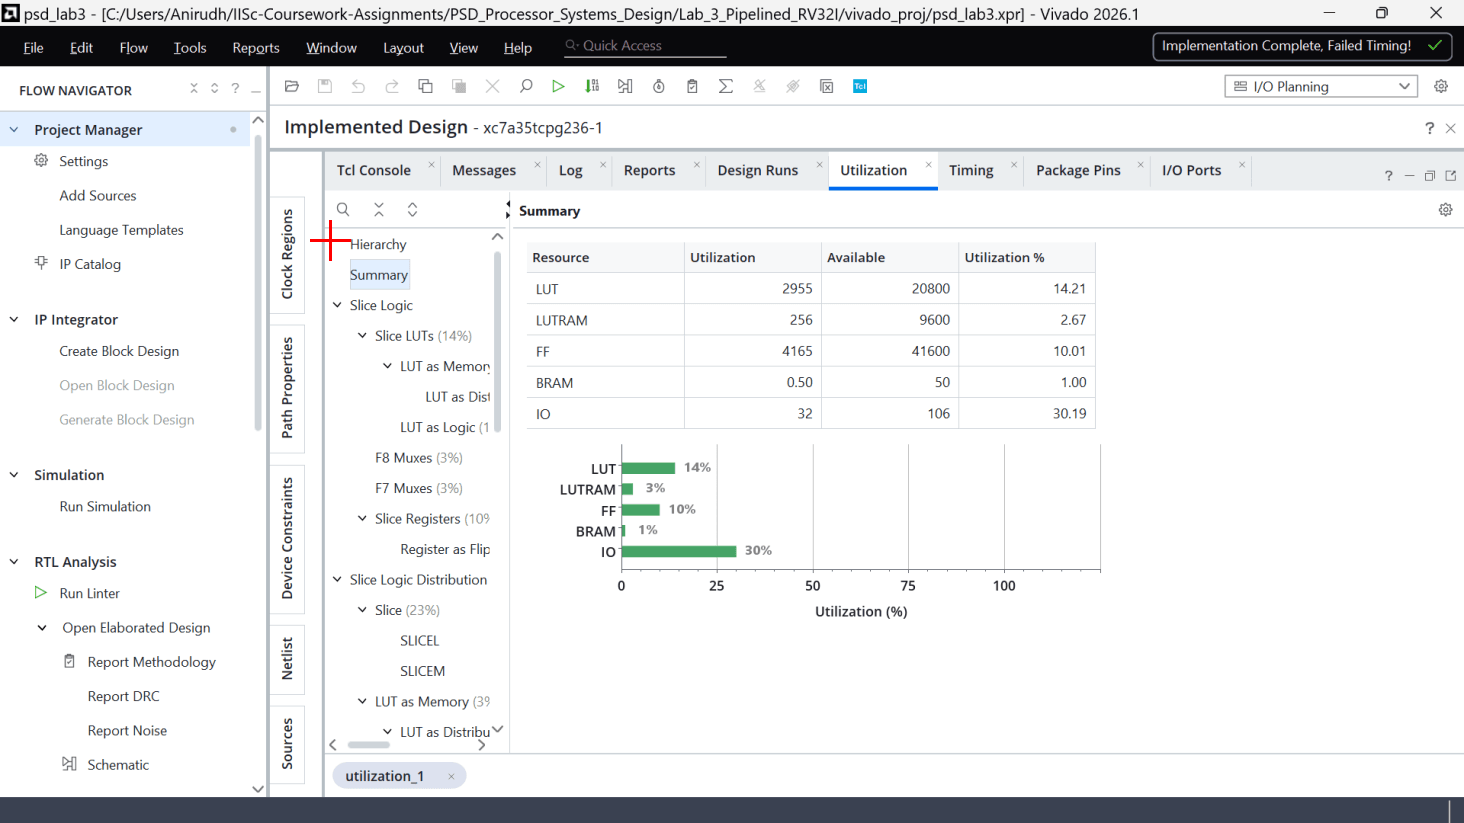
\includegraphics[width=0.9\textwidth]{figures/fig_util.png}
\caption{Vivado post-route utilization summary: 2,955 LUTs (14.21\%), 256 LUTRAM (2.67\%), 4,165 flip-flops (10.01\%), 0.5 BRAM tile (1.00\%), 32 I/O (30.19\%).}
\label{fig:util}
\end{figure}

\begin{figure}[htbp]
\centering
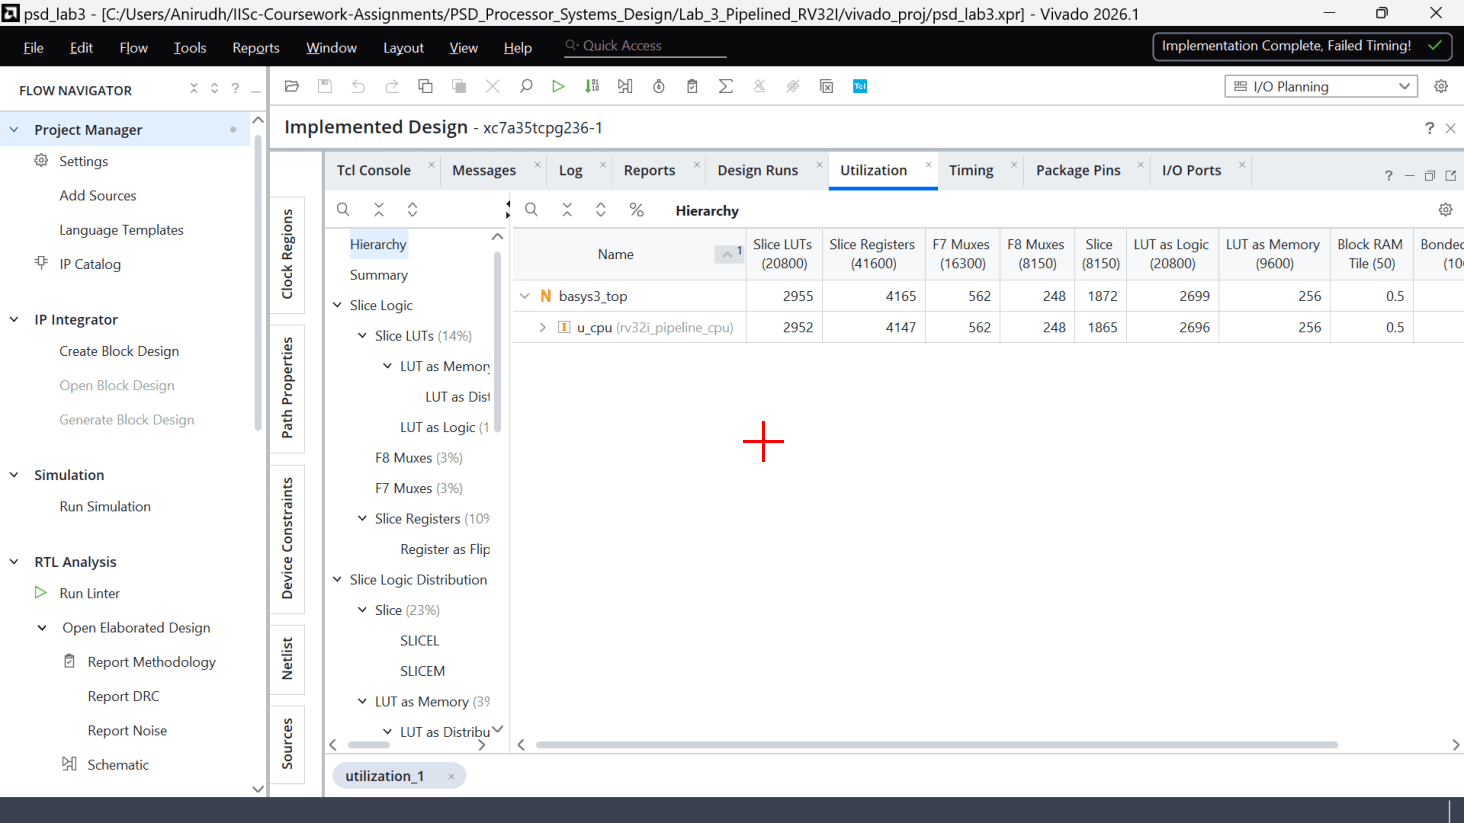
\includegraphics[width=\textwidth]{figures/fig_util_hier.png}
\caption{Post-route utilization by hierarchy: \texttt{u\_cpu} accounts for 2,952 of the 2,955 LUTs and 4,147 of the 4,165 registers.}
\label{fig:utilhier}
\end{figure}

\subsection*{Timing analysis}
\begin{figure}[htbp]
\centering
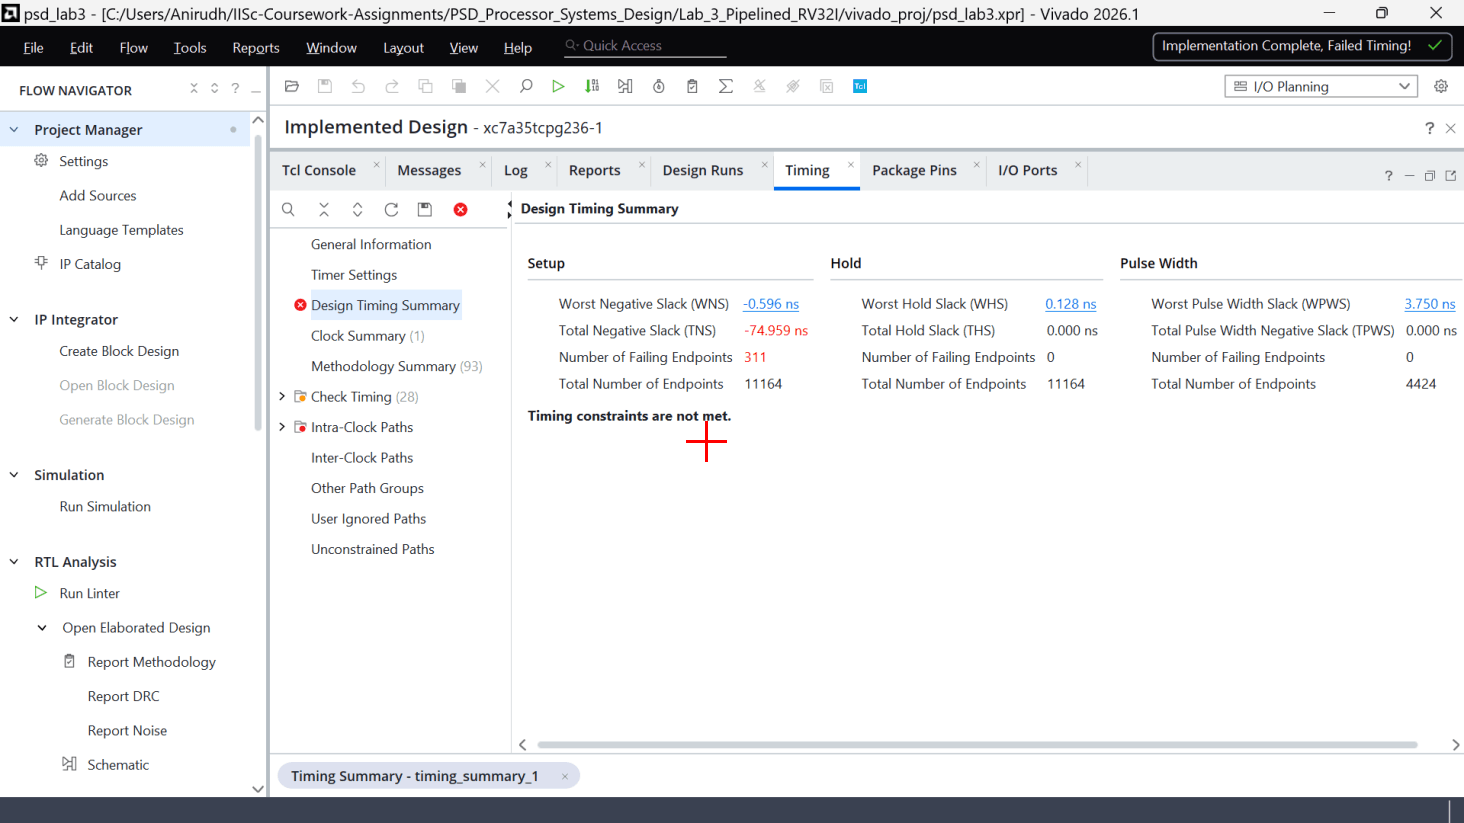
\includegraphics[width=\textwidth]{figures/fig_timing_summary.png}
\caption{Vivado Design Timing Summary at the 10~ns (100~MHz) constraint: WNS $=-0.596$~ns, TNS $=-74.959$~ns with 311 failing setup endpoints out of 11,164; WHS $=+0.128$~ns (0 failing); WPWS $=3.750$~ns. Vivado reports ``Timing constraints are not met''.}
\label{fig:timing}
\end{figure}

\begin{figure}[htbp]
\centering
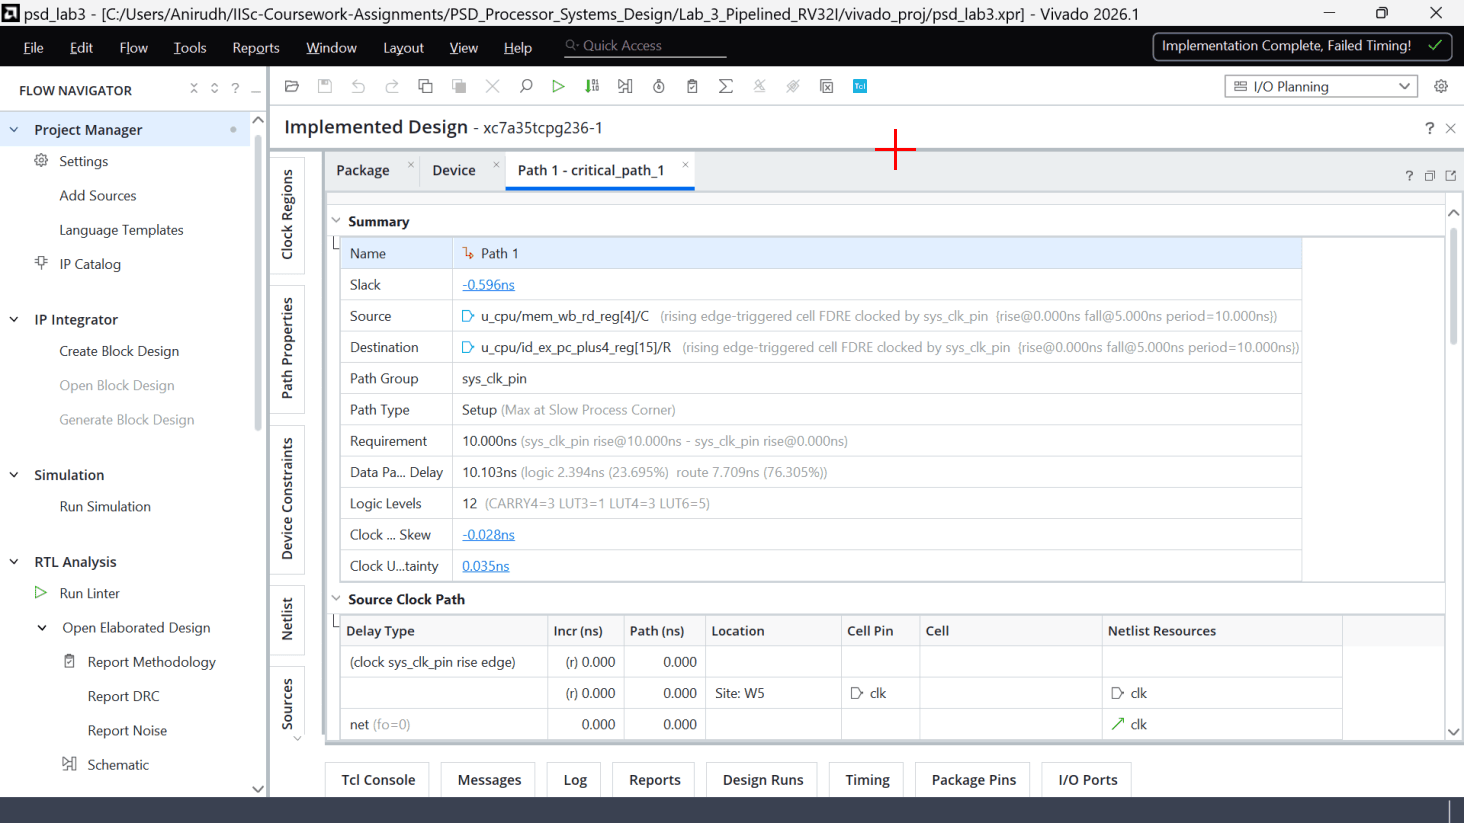
\includegraphics[width=\textwidth]{figures/fig_critical_path_detail.png}
\caption{Worst setup path (Slow process corner): from \texttt{u\_cpu/mem\_wb\_rd\_reg[4]} to the reset pin of \texttt{u\_cpu/id\_ex\_pc\_plus4\_reg[15]}. Data-path delay 10.103~ns, of which logic 2.394~ns (23.7\%) and routing 7.709~ns (76.3\%); 12 logic levels (CARRY4 $\times$3, LUT3 $\times$1, LUT4 $\times$3, LUT6 $\times$5).}
\label{fig:critpath}
\end{figure}

The design does \textbf{not} meet the 100~MHz constraint: the worst setup slack is $-0.596$~ns, so the maximum frequency supported by static timing analysis is about $1/(10.000+0.596)~\text{ns} \approx 94.4$~MHz. Hold and pulse-width checks pass.

The worst path (Figure~\ref{fig:critpath} and the full path in \texttt{reports/rebuild/post\_route\_timing.rpt}) starts at the write-back register \texttt{mem\_wb\_rd}, passes through the forwarding select logic into \texttt{ex\_op\_a\_fwd}, then through the branch comparator's carry chain (\texttt{u\_branch}) to \texttt{ex\_branch\_cond}, \texttt{ex\_redirect} and the load-use/stall logic, and finally fans out (fanout 190) to the synchronous reset of the ID/EX pipeline registers. In other words it is the \emph{forward $\rightarrow$ compare $\rightarrow$ redirect $\rightarrow$ flush} chain inside the EX stage, and 76\% of its delay is routing rather than logic.

Ways to shorten it, which were not implemented in this submission, would be to register part of the redirect decision, reduce the fanout of the ID/EX flush signal (replicate it or use clock enables), or simply constrain the clock to about 10.6~ns (94~MHz).

The post-route timing simulation in the previous section passes at the 10~ns clock. That does not contradict the failing slack: the simulation only exercises the paths this particular program sensitises, whereas static timing analysis checks every path at the slow process corner. The correct statement of the achieved performance is therefore the static-timing result above, not 100~MHz.

\appendix
\section{C code}
\lstinputlisting[language=C]{../memory/restoring_div.c}

\section{Assembly code}
\lstinputlisting{../memory/restoring_div.asm}

\section{Constraint file (\texttt{basys3.xdc})}
\lstinputlisting{../constrs/basys3.xdc}

\section{Key Verilog sources}
The complete source files are in the \texttt{rtl/} folder: \texttt{rv32i\_pipeline\_cpu.v}, \texttt{icache.v}, \texttt{instr\_bram.v}, \texttt{hazard\_unit.v}, \texttt{forwarding\_unit.v}, \texttt{branch\_unit.v}, \texttt{alu.v}, \texttt{control\_unit.v}, \texttt{imm\_gen.v}, \texttt{reg\_file.v}, \texttt{data\_mem.v}, \texttt{seg7\_driver.v}, \texttt{basys3\_top.v}, \texttt{rv32i\_defines.v}. The testbenches are in \texttt{testbench/}. The three modules that implement the stall, forwarding and cache behaviour shown in the waveforms are listed below.

\subsection*{\texttt{hazard\_unit.v}}
\lstinputlisting[language=Verilog]{../rtl/hazard_unit.v}

\subsection*{\texttt{forwarding\_unit.v}}
\lstinputlisting[language=Verilog]{../rtl/forwarding_unit.v}

\subsection*{\texttt{icache.v}}
\lstinputlisting[language=Verilog]{../rtl/icache.v}

\end{document}
